\documentclass[12pt]{article}

\usepackage[T2A]{fontenc}
\usepackage[utf8]{inputenc}
\usepackage[english,russian]{babel}

\usepackage{amsmath,amsfonts,amssymb,amsthm,mathtools}

\usepackage[figurename=Рисунок]{caption}

\usepackage{geometry} % Простой способ задавать поля
\geometry{top=20mm}
\geometry{bottom=20mm}
\geometry{left=25mm}
\geometry{right=25mm}
\pagestyle{empty}

\usepackage{graphicx} % Для вставки рисунков 
\graphicspath{{images/}{images2/}} % папки с картинками 
\DeclareGraphicsExtensions{.pdf,.png,.jpg}
\setlength\fboxsep{3pt} % Отступ рамки \fbox{} от рисунка 
\setlength\fboxrule{1pt} % Толщина линий рамки \fbox{} 
\usepackage{wrapfig} % Обтекание рисунков и таблиц текстом


\begin{document}
%начало титульного листа
\begin{titlepage}
\newpage
\begin{center}
\vspace{1cm}%расстояние до верхней строчки
\LARGE Московский Физико-Технический\\ Институт \\*
\vspace{5mm}
\large Факультет Биологической и Медицинской Физики\\*
\hrulefill %горизонтальная черта
\end{center}
\vspace{5em}
\begin{center}
\textbf{\huge Основы MALDI-TOF масс-спектрометрии} 
\end{center}
\vspace{20em}
\begin{flushright}
Выполнили: 
\hspace{1em}  
Яновская Дарья (6112)\\
Михайлова Анна (6112)\\
Колосов Семен (6112)\\
\vspace{1.5em}
\end{flushright}
\vspace{\fill}
\begin{center}
Москва 2019
\end{center}
\end{titlepage}
%конец титульного листа
 
\newpage

\begin{flushleft}
\section{ Цели работы}
%\vspace{1.5em}
\begin{itemize}
\item Получение масс-спектра смеси пептидов с и без рефлектрона.
\item Определение зависимости основных аналичических характеристик от энергии лазера.
\item Определение зависимости основных аналичических характеристик от длительности ускоряющего напряжения.
\item Определение зависимости основных аналичических характеристик от длительности импульса.
\end{itemize}

\section{Теоретическая часть}
\subsection{Метод ионизации MALDI}
Масс-спектрометр - прибор для химических исследований. Анализируемые молекулы (аналиты) сначала ионизируют в вакууме. Затем вновь
образовавшиеся заряженные частицы вводятся в электрическое и (или) магнитное поле,
причем их движение в поле зависит от отношения их массы к заряду $(m/z)$. Эта измеряемая величина может быть использована для определения молекулярной массы
аналита с высокой точностью.\\
\vspace{1em}
В данной работе для исследования высокомолекулярных исследований используется метод ионизации MALDI (Matrix Assisted
Laser Desorption/Ionization) вместе с времяпролётным масс-анализатором (TOF — time
of flight). Особенностью данного метода является перевод вещества из конденсированного состояния в газовую фазу под воздействием лазерного излучения, что позволяет провести «мягкую» ионизацию. Наиболее эффективно облучать исследуемое вещество
в смеси с другим веществом —  матрицей. Матрица адсорбирует (поглощает) энергию излучения лазера, что предотвращает разрушение анализируемых молекул. \\
\vspace{1em}
Чтобы приготовить образец для массспектрометрического анализа MALDI, нужно растворить аналит и матрицу в
подходящем растворителе с последующей сокристаллизации указанных компонентов на
металлической подложке (мишени). При переходе в твердую фазу растворитель испаряется и происходит сокристаллизация. При освещении лазером высокая при низком давлении (около 0.75 торр)
плотность энергии в точке облучения приводит к взрывному испарению матрицы, которая
включает в себя следы анализируемого соединения. В результате над мишенью образуется облако ионов и незаряженных частиц с начальными скоростями от 400 до 800 м/с. Нейтральные частицы удаляются турбомолекулярным насосом, а ионы вытягиваются разницей потенциалов, приложенной между мишенью и фокусирующими линзами.\\
\textbf{Масс-спектр} — это зависимость интенсивности ионного тока (количества вещества) от
отношения массы к заряду.
\newpage
Процесс ионизации в MALDI состоит из двух стадий:
\begin{enumerate}
\item Первая стадия (\textbf{первичная ионизация}) — образование первичных свободных ионов из молекул матрицы(фазовый переход твердое тело - газ). \textbf{Абляция} - процесс взрывного испарения твердого тела при перегревании высоко-интенсивным лазерным излучением.
\item Вторая стадия (\textbf{вторичная ионизация})— формирование ионов анализируемого вещества в газовой фазе в
результате взаимодействия ионов матрицы и нейтральных молекул анализируемого
вещества (ион-молекулярных процессы).
\end{enumerate}
\textbf{Десорбция} - плавный переход от твердого тела к газовой фазе вблизи поверхности образца. Происходит обеих стадиях.
\subsection{MALDI-TOF масс-спектрометрия}
Схема масс-спектрометра состоит из области с высоким значением $E$ напряженности электрического поля и бесполевой области дрейфа. Ускоряющее напряжение $U=E\cdot s$.
Время $t$ движения иона от момента начала лазерного импульса
до момента попадания иона на детектор следующим образом зависит от величины $\sqrt{m/z}$:
\[ t= \sqrt{m/z}\cdot const + t_0
\]
где const и $t_0$ определяются длиной полевой области, длиной бесполевой области (области дрейфа), расстоянием от места образования иона до поверхности образца, начальной
кинетической энергии иона, разностью потенциалов и временем от момента начала лазерного импульса до момента образования ионы.
\begin{figure}[!h]
\center{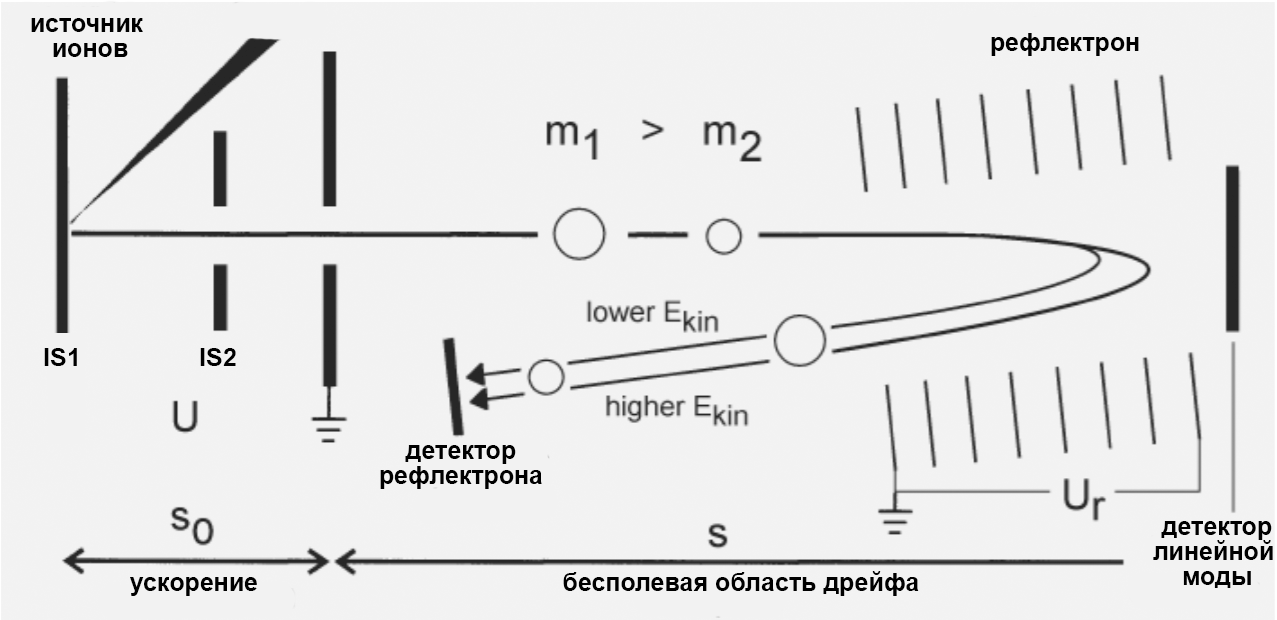
\includegraphics[width=14cm,height=8cm]{1}}
\caption{MALDI-TOF масс-спектрометр с рефлектроном.}
\label{ris:image}
\end{figure}

\subsubsection{Метод импульсной экстракции ионов PIE}

В процессе PIE участвуют мишень(IS1) с образцом, пластина вторичного напряжения(IS2) и заземленный ускоряющий электрод.\\
\textbf{На первом этапе} на IS1 и IS2 потенциял $\phi_1$ и аналит не подвергается воздействию внешних эффектов до удара лазерного луча.\\
\textbf{На втором этапе} в факеле происходит ионизация аналита и тепловой дрейф ионов от IS1 к IS2. Из за теплового разброса у них разная начальная скорость.\\
\textbf{На третьем этапе} после некоторого времени задержки $t_{delay}$ потенциал IS2 снижается до $\phi_2$, создавае поле, которое заставляет все заряженные частицы двигаться к IS2. В результате ионы с заданной массой и различными начальными скоростями достигнут детектора одновременно.\\
Свойства:
\begin{enumerate}
\item оптимальное время задержки зависит от $(m/z)$ т.е. эффективная фокусировка ионов осуществляется для узкого диапазона $(m/z)$
\item оины с большими массами лучше фокусируются при увеличении амплитуды выталкивающего импульса и $t_{delay}=const$
\item время задержки уменьшается с увеличением амплитуды выталкивающего импульса
\end{enumerate}
\subsubsection{Рефлектрон}

При помощи электростатического поля ионы отражаются под небольшим углом в направлении детектора рефлектрона. Ионы с большей кинетической энергией проникают глубже внутрь поля рефлектрона, тратя больше времени на замедление и последующее ускорение. Достигая ионного зеркала первыми, они последними покидают его и догоняют более медленные ионы.\\
Свойстава:
\begin{enumerate}
\item фокусировка ионов не зависит от массы
\item нельзя использовать для анализа больших белков
\end{enumerate}
\subsubsection{Порог чуствительности и разрешающая способность}
\textbf{Порог чувствительности} определяется минимальным количеством молекул образца, которое  дает детектируемый ионный сигнал в масс-спектре (в диапазоне наномолей для пептидов и в диапазоне микромолей для белков).\\
\textbf{Разрешающая способность} определяется как $R=\frac{x}{\Delta x}$,
где $\Delta x$ — расстояние между максимально близко стоящими пиками, но тем не менее различными, а $x$ — характерная величина координаты этих пиков. 
\subsection{Изотопное распределение}
Разные атомы одного элемента могут иметь разную массу из-за разного количества нейтронов в ядре - изотопы.\\
\textbf{Изотопные пики} - пики, сооьветствующие ионам с одной химической формулой, но разным изотопным составом. Если разрешение прибора высокое, можно увидеть тонкую изотопную структуру, где каждому изотопу соответствует свой пик. Иначе, пики сливаются в один.При заряде иона 1 расстояние между изотопными пиками $m/z = 1$ ,при заряде 2 - $m/z = 0.5$ и тд.\\
\textbf{Моноизотопные пики} - все атомы, входящие в состав, одной массы.
\section{Экспериментальная часть}
\subsection{Определение зависимости аналитических характеристик метода от мощности лазерного излучения при Default linear}

Сняли спектры смеси пептидов при значениях мощности лазера от 0 до 100 с шагом 10. \\
Ниже 20 вообще не видели никакого масс-спектра. От 20 до 40 виден только шум. Выше 40 стали различимы пики.
\begin{figure}[!h]
\center{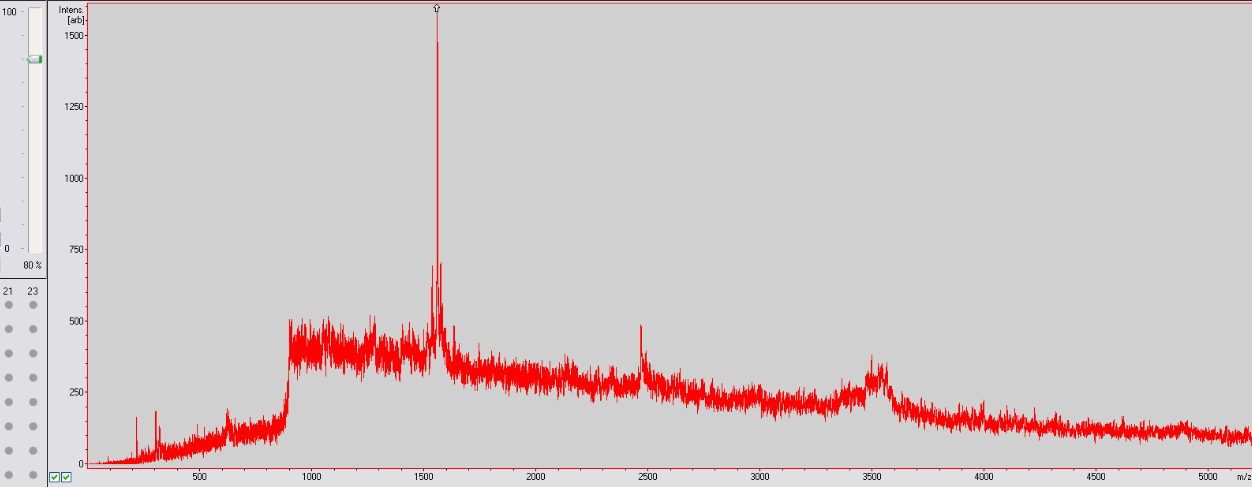
\includegraphics[width=14cm,height=8cm]{9}}
\caption{Спектр при мощности лазера 80, на которой лучше всего видны пики.}
\label{ris:image}
\end{figure}
\newpage
\begin{figure}[!h]
\begin{center}
\begin{minipage}[h]{0.4\linewidth}
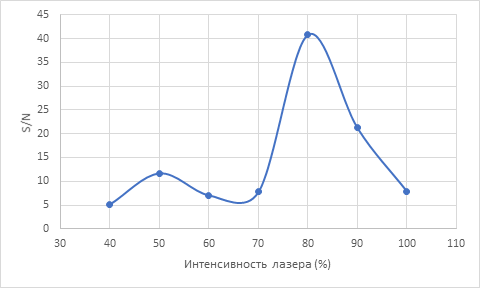
\includegraphics[width=1.2\linewidth]{3}
\caption{Зависимость значений $S/N$ от мощности лазерного излучения
для пика 1557 Да.} %% подпись к рисунку
\label{ris:experimoriginal} %% метка рисунка для ссылки на него
\end{minipage}
\hfill 
\begin{minipage}[h]{0.4\linewidth}
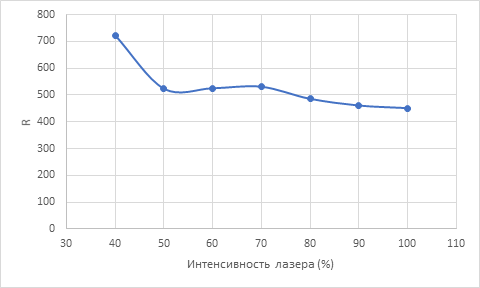
\includegraphics[width=1.2\linewidth]{4}
\caption{Зависимость разрешения пиков от
мощности лазерного излучения для пика 1557 Да.}
\label{ris:experimcoded}
\end{minipage}
\end{center}
\end{figure}
\subsection{Определение зависимости аналитических характеристик метода от мощности лазерного излучения при Default reflectron}
Сняли спектры смеси пептидов при различных значениях
мощности лазера на методе с рефлектроном. Пики различимы с 60. Наилучшее соотношение сигнал/шум при мощности 80. Также наблюдается уменьшение разрешения пиков при увеличении мощности лазера. Это можно
объяснить тем, что происходит фрагментация молекул, а также присутствует больший
тепловой разброс по скоростям.
\begin{figure}[!h]
\center{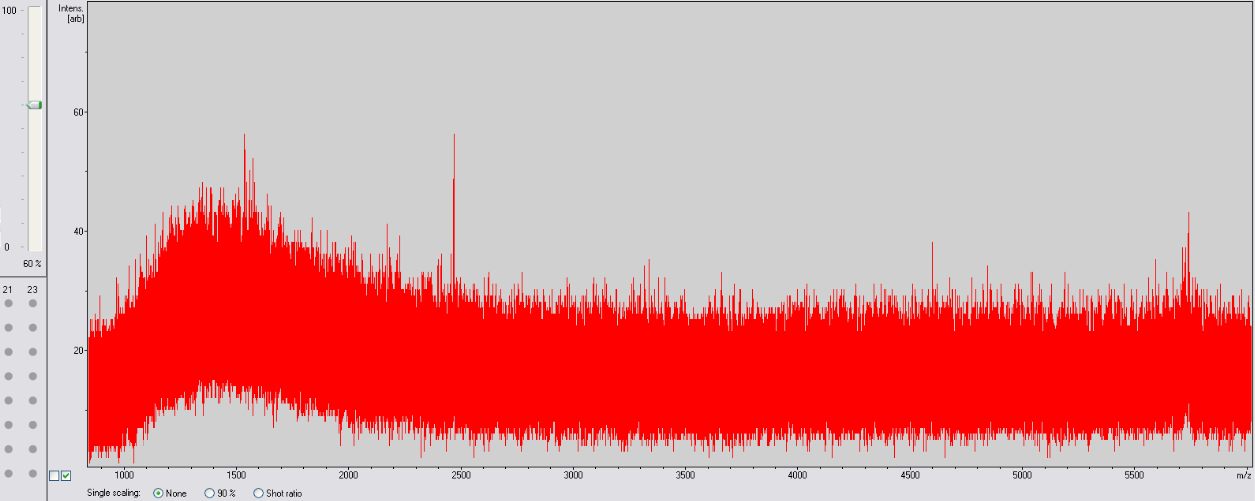
\includegraphics[width=14cm,height=8cm]{10}}
\caption{Спектр при мощности лазера 60 с рефлектроном.}
\label{ris:image}
\end{figure}
\newpage
\subsection{Определение влияния времени включения ускоряющего потенциала на масс-спектр в режиме без рефлектрона}
Снимем спектры смеси пептидов при различных значениях времени включения ускоряющего потенциала (от 0 нс до 500 нс) и построим графики зависимости значений S/N (отношение сигнал/шум) и разрешения
основных пиков от времени включения ускоряющего потенциала.
\begin{figure}[!h]
\begin{center}
\begin{minipage}[h]{0.4\linewidth}
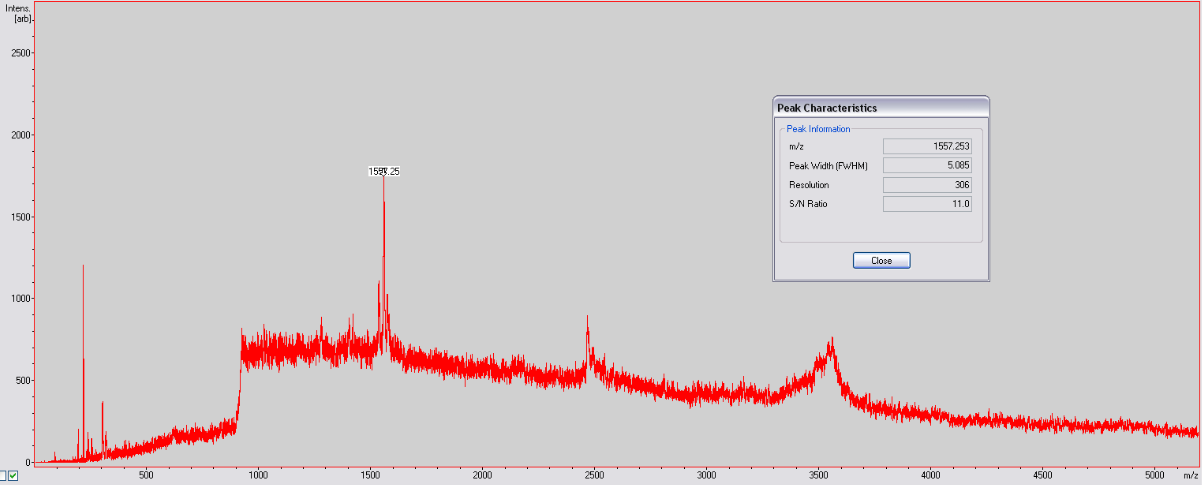
\includegraphics[width=1.2\linewidth]{11}
\caption{Спектр при t=0 нс.} %% подпись к рисунку
\label{ris:experimoriginal} %% метка рисунка для ссылки на него
\end{minipage}
\hfill 
\begin{minipage}[h]{0.4\linewidth}
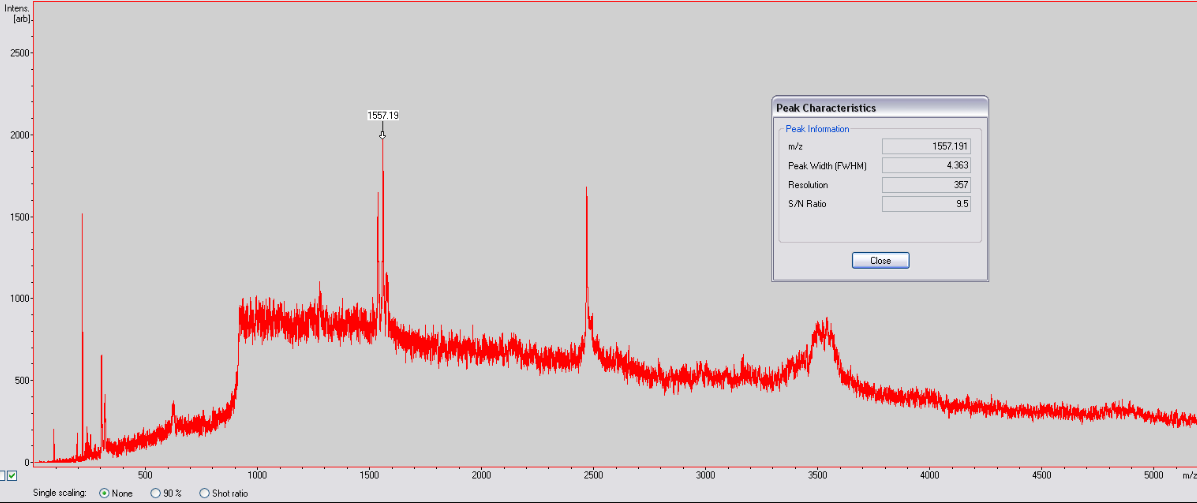
\includegraphics[width=1.2\linewidth]{12}
\caption{Спектр при t=40 нс.}
\label{ris:experimcoded}
\end{minipage}
\end{center}
\end{figure}

\begin{figure}[!h]
\begin{center}
\begin{minipage}[h]{0.4\linewidth}
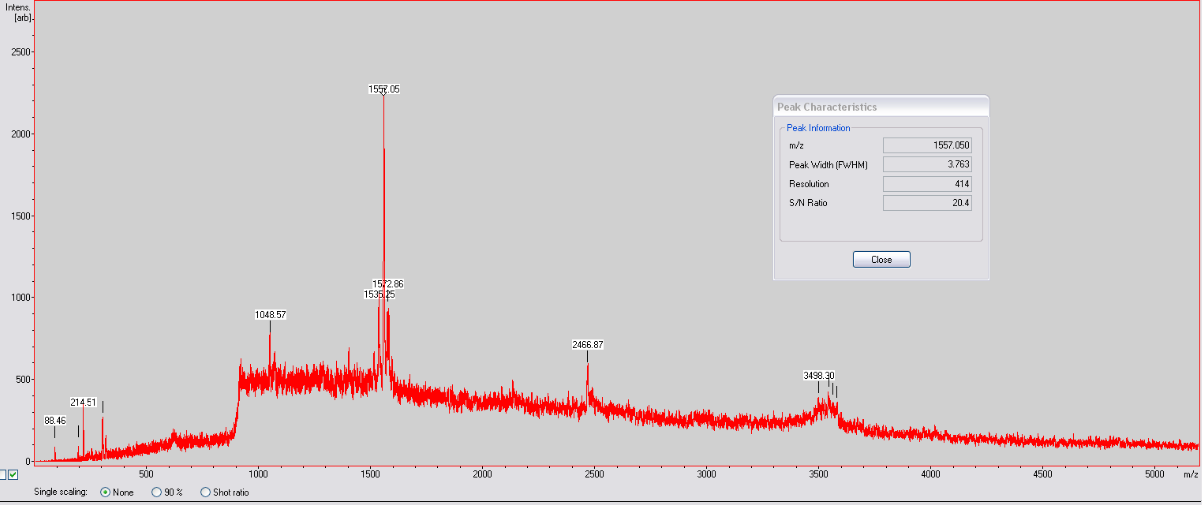
\includegraphics[width=1.2\linewidth]{13}
\caption{Спектр при t=80 нс.} %% подпись к рисунку
\label{ris:experimoriginal} %% метка рисунка для ссылки на него
\end{minipage}
\hfill 
\begin{minipage}[h]{0.4\linewidth}
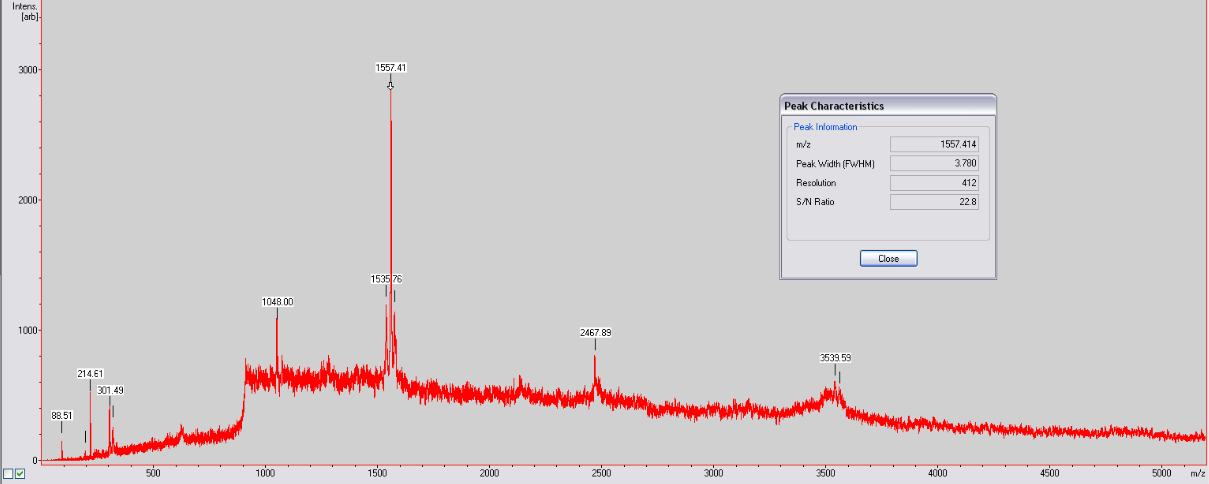
\includegraphics[width=1.2\linewidth]{14}
\caption{Спектр при t=120 нс.}
\label{ris:experimcoded}
\end{minipage}
\end{center}
\end{figure}

\begin{figure}[!h]
\begin{center}
\begin{minipage}[h]{0.4\linewidth}
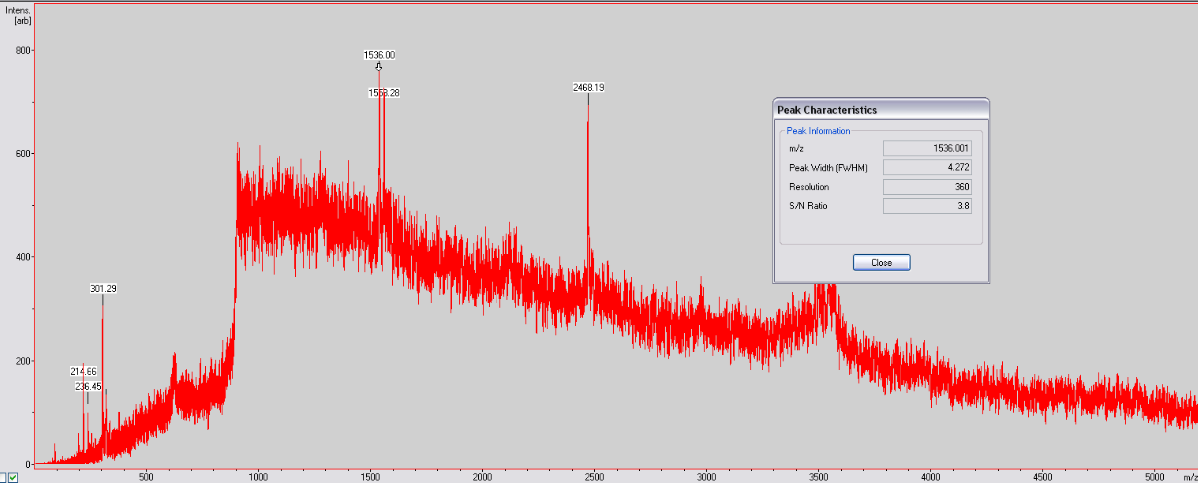
\includegraphics[width=1.2\linewidth]{15}
\caption{Спектр при t=180 нс.} %% подпись к рисунку
\label{ris:experimoriginal} %% метка рисунка для ссылки на него
\end{minipage}
\hfill 
\begin{minipage}[h]{0.4\linewidth}
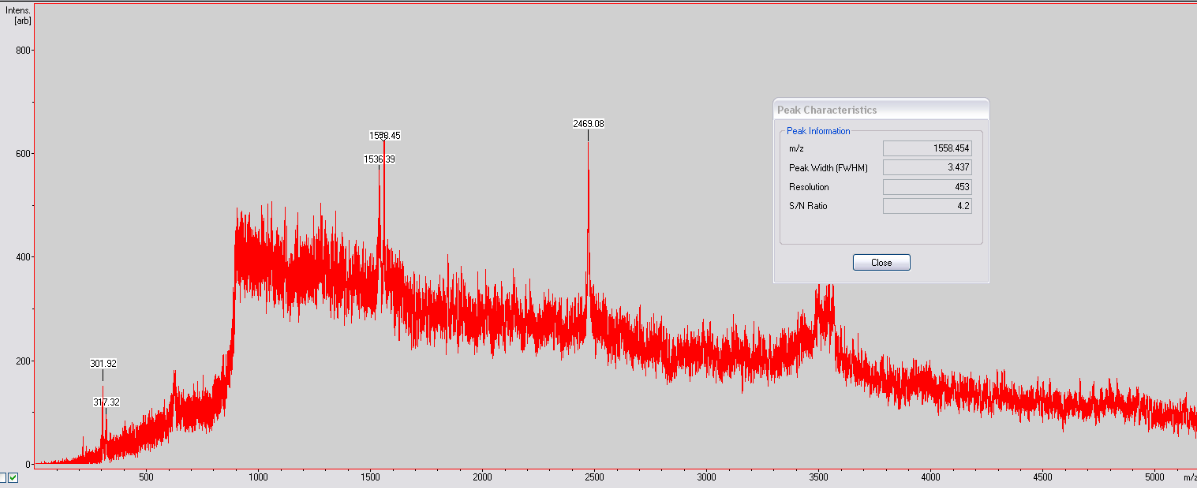
\includegraphics[width=1.2\linewidth]{16}
\caption{Спектр при t=250 нс.}
\label{ris:experimcoded}
\end{minipage}
\end{center}
\end{figure}
\newpage

\begin{figure}[!h]
\begin{center}
\begin{minipage}[h]{0.4\linewidth}
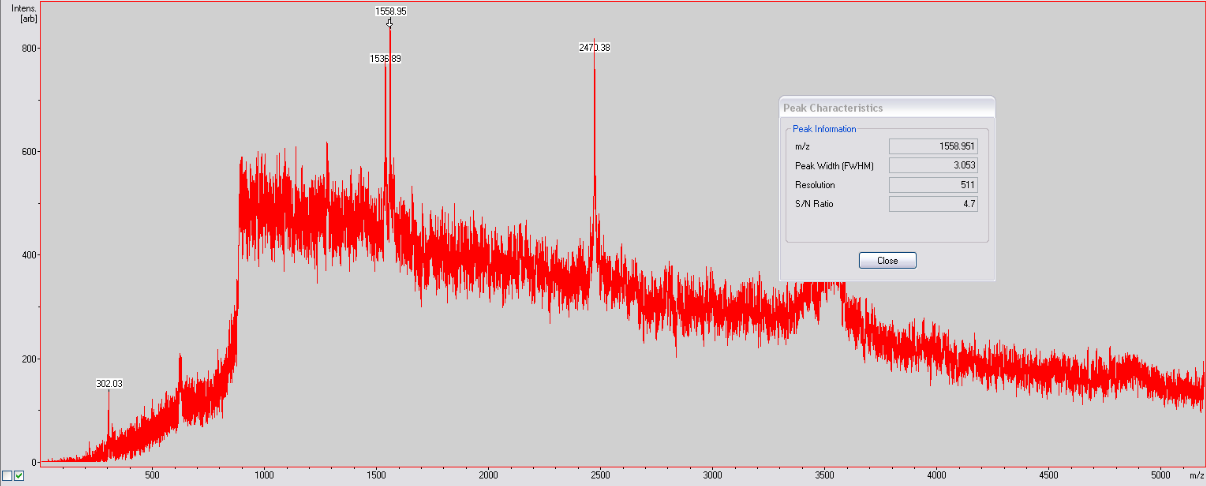
\includegraphics[width=1.2\linewidth]{17}
\caption{Спектр при t=330 нс.} %% подпись к рисунку
\label{ris:experimoriginal} %% метка рисунка для ссылки на него
\end{minipage}
\hfill 
\begin{minipage}[h]{0.4\linewidth}
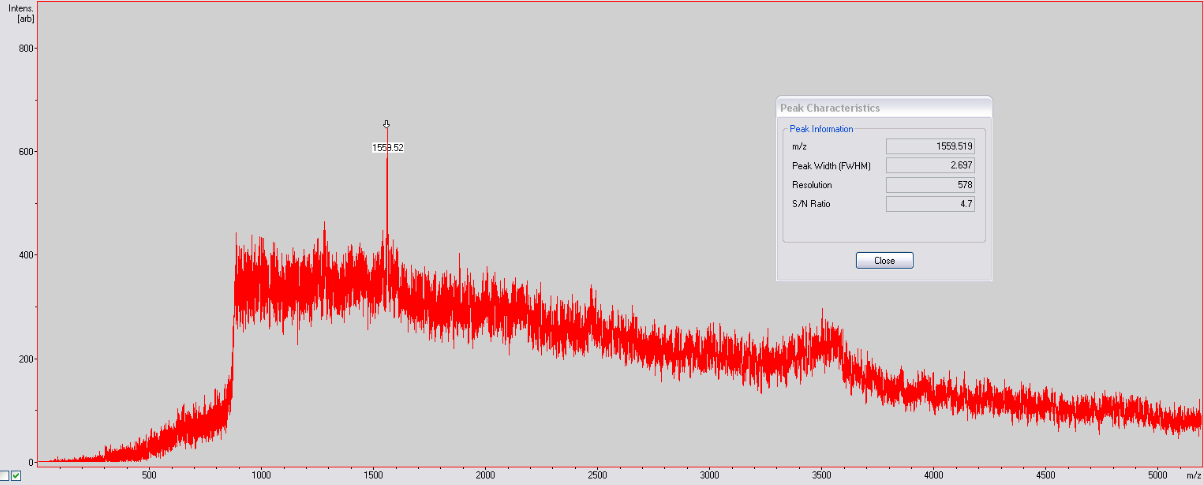
\includegraphics[width=1.2\linewidth]{18}
\caption{Спектр при t=410 нс.}
\label{ris:experimcoded}
\end{minipage}
\end{center}
\end{figure}

\begin{figure}[!h]
\center{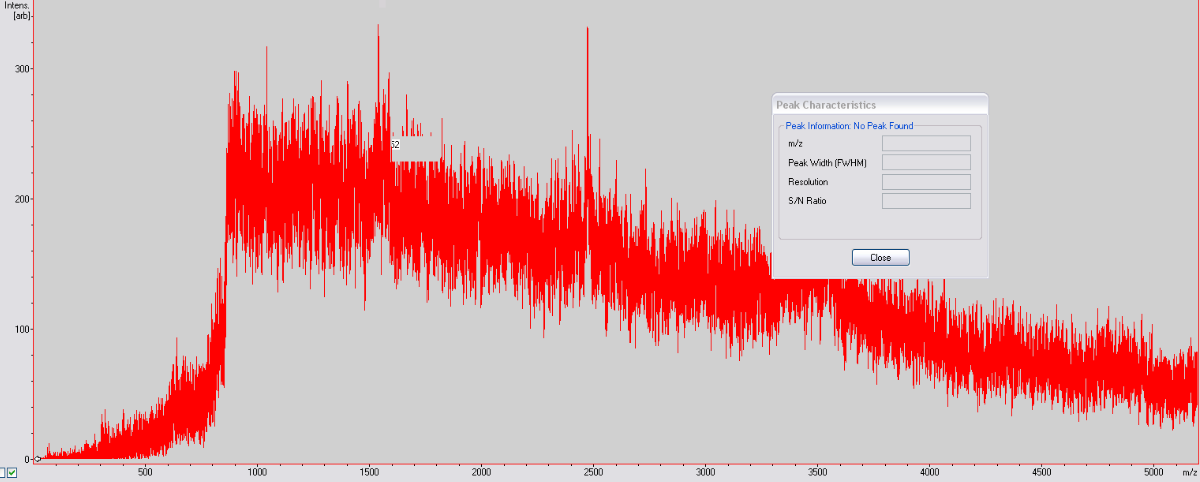
\includegraphics[width=14cm,height=6cm]{19}}
\caption{Спектр при t=500 нс.}
\label{ris:image}
\end{figure}

\begin{figure}[!h]
\begin{center}
\begin{minipage}[h]{0.4\linewidth}
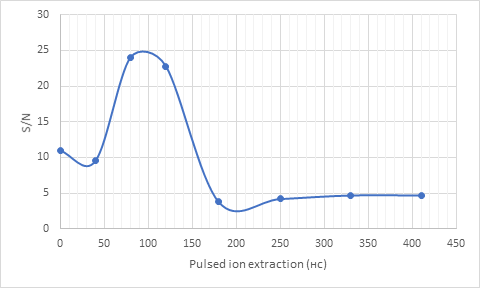
\includegraphics[width=1.2\linewidth]{7}
\caption{Зависимость значений S/N от времени включения ускоряющего потенциала без рефлектрона.} %% подпись к рисунку
\label{ris:experimoriginal} %% метка рисунка для ссылки на него
\end{minipage}
\hfill 
\begin{minipage}[h]{0.4\linewidth}
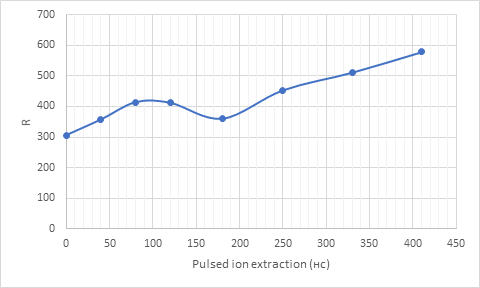
\includegraphics[width=1.2\linewidth]{8}
\caption{Зависимость разрешения пиков от времени включения ускоряющего потенциала без рефлектрона.}
\label{ris:experimcoded}
\end{minipage}
\end{center}
\end{figure}

Исходя из графика, можно предположить, что при увеличении
времени включения ускоряющего потенциала всё больше частиц успевает
откачаться насосами, в том числе и источники шума. Количество
ионов аналита, имеющих достаточную энергию для вылета в дрейфовую
зону, падает сильно, что и приводит к уменьшению значения S/N.
\subsection{Определение влияния времени включения ускоряющего потенциала на масс-спектр в режиме с рефлектроном}
Снимали спектры смеси пептидов при значениях времени включения ускоряющего потенциала от 0 нс до 250 нс. При увеличении времени пики пропадают и остается только шум.
\begin{figure}[!h]
\begin{center}
\begin{minipage}[h]{0.4\linewidth}
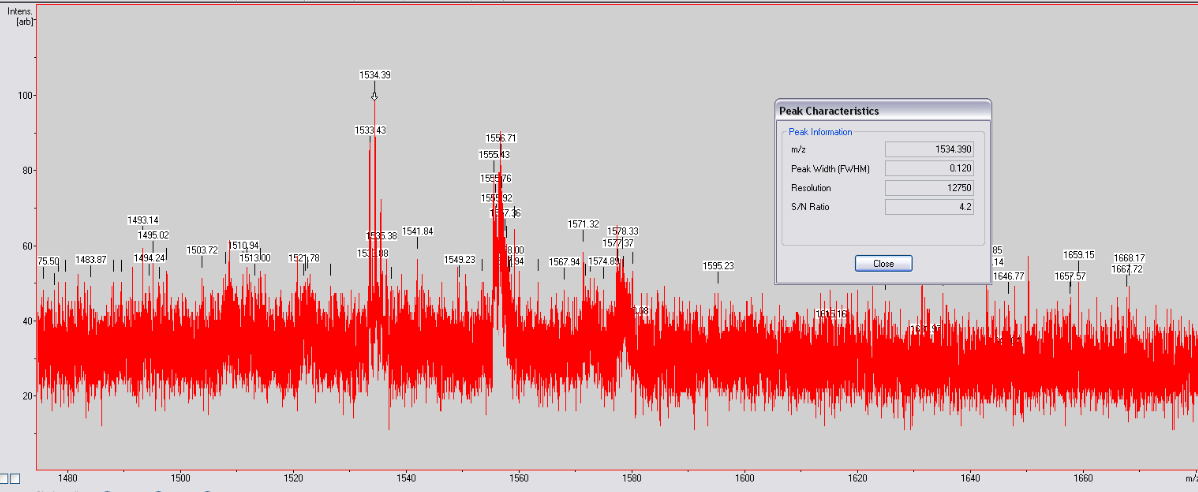
\includegraphics[width=1.2\linewidth]{20}
\caption{Спектр при t=0 нс.} %% подпись к рисунку
\label{ris:experimoriginal} %% метка рисунка для ссылки на него
\end{minipage}
\hfill 
\begin{minipage}[h]{0.4\linewidth}
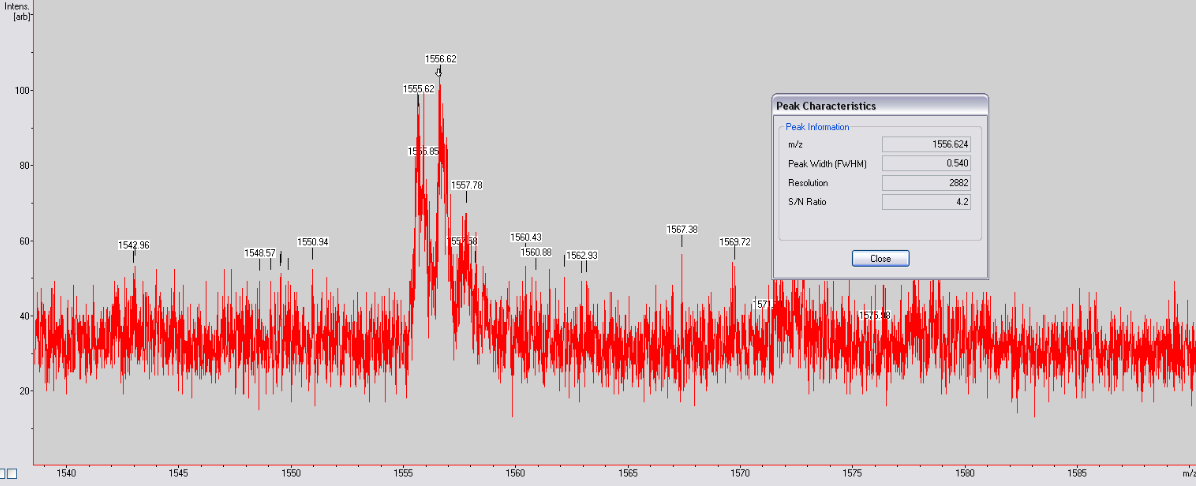
\includegraphics[width=1.2\linewidth]{21}
\caption{Спектр при t=40 нс.}
\label{ris:experimcoded}
\end{minipage}
\end{center}
\end{figure}

\begin{figure}[!h]
\begin{center}
\begin{minipage}[h]{0.4\linewidth}
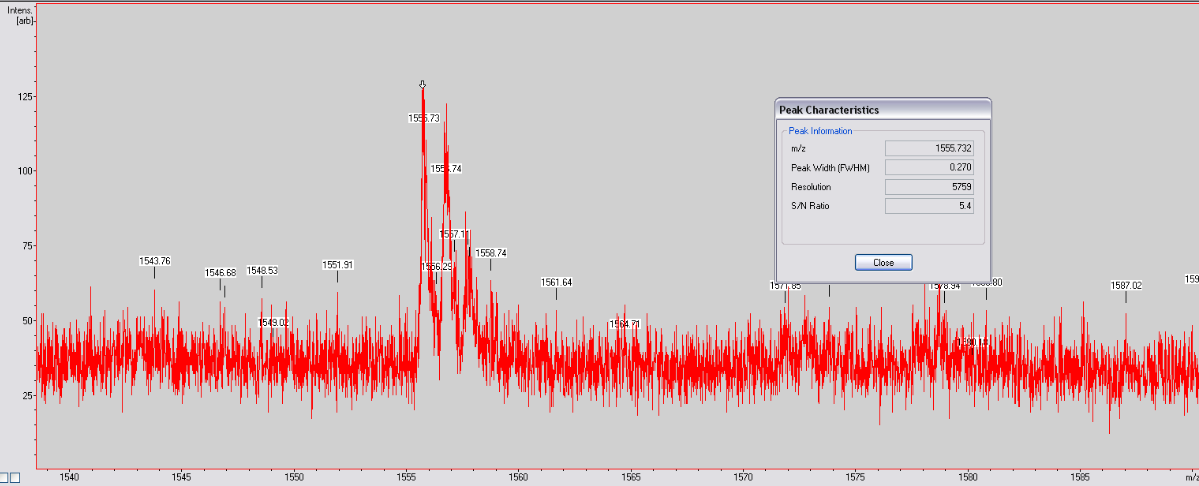
\includegraphics[width=1.2\linewidth]{22}
\caption{Спектр при t=80 нс.} %% подпись к рисунку
\label{ris:experimoriginal} %% метка рисунка для ссылки на него
\end{minipage}
\hfill 
\begin{minipage}[h]{0.4\linewidth}
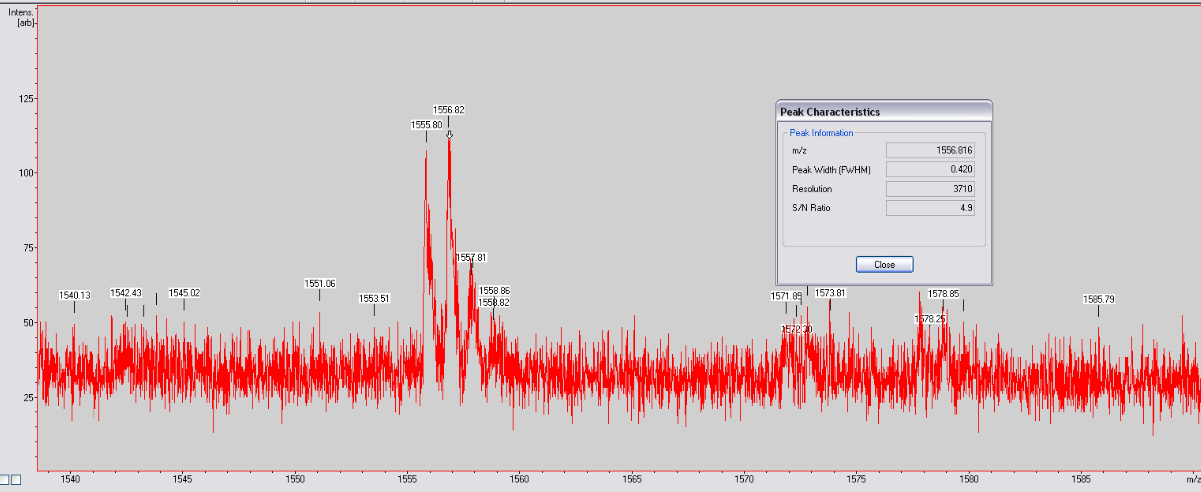
\includegraphics[width=1.2\linewidth]{23}
\caption{Спектр при t=120 нс.}
\label{ris:experimcoded}
\end{minipage}
\end{center}
\end{figure}

\begin{figure}[!h]
\begin{center}
\begin{minipage}[h]{0.4\linewidth}
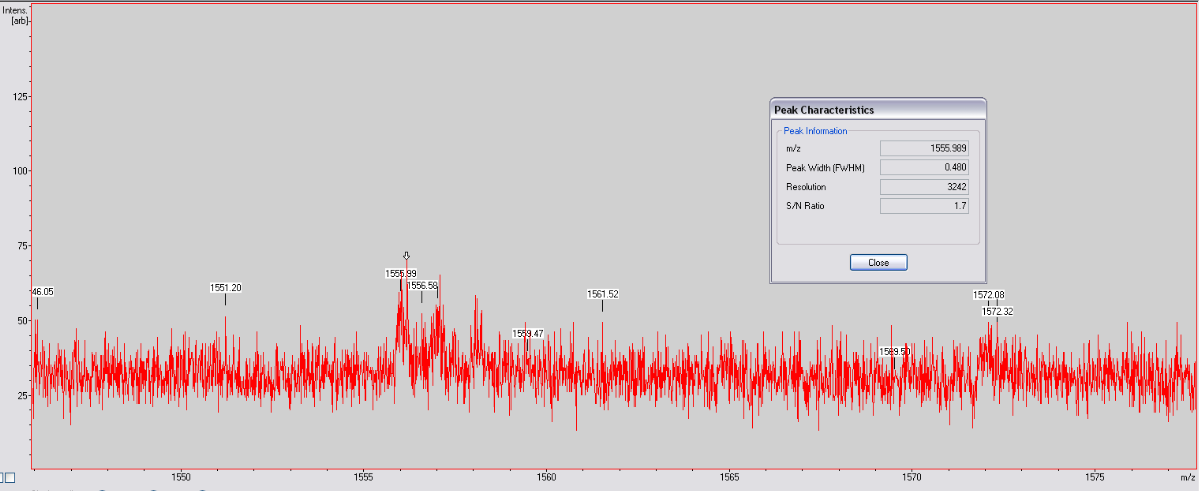
\includegraphics[width=1.2\linewidth]{24}
\caption{Спектр при t=180 нс.} %% подпись к рисунку
\label{ris:experimoriginal} %% метка рисунка для ссылки на него
\end{minipage}
\hfill 
\begin{minipage}[h]{0.4\linewidth}
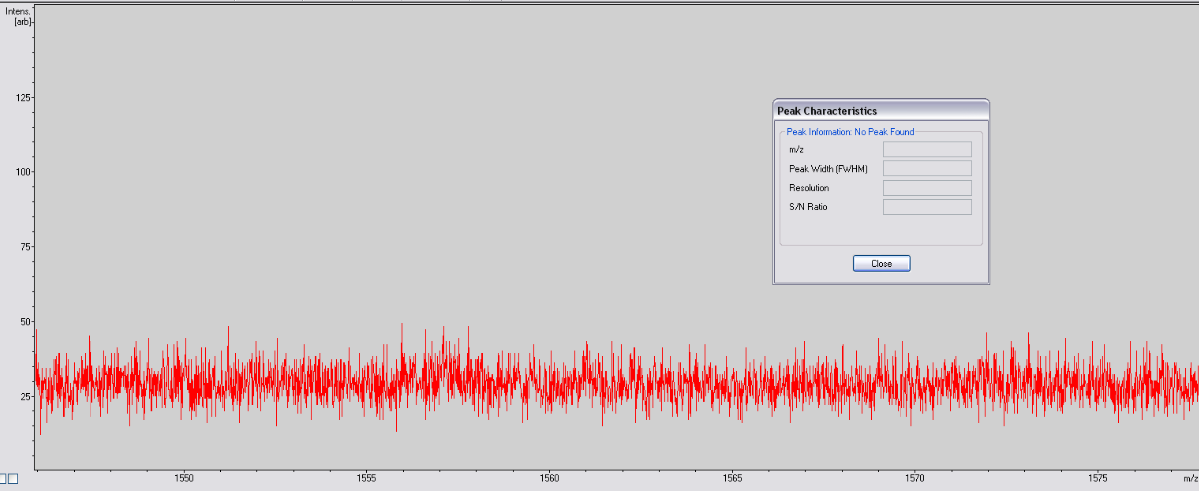
\includegraphics[width=1.2\linewidth]{25}
\caption{Спектр при t=250 нс.}
\label{ris:experimcoded}
\end{minipage}
\end{center}
\end{figure}
\newpage

\begin{figure}[!h]
\begin{center}
\begin{minipage}[h]{0.4\linewidth}
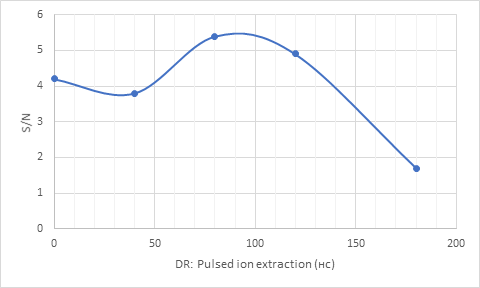
\includegraphics[width=1.2\linewidth]{5}
\caption{Зависимость значений S/N от времени включения ускоряющего потенциала с рефлектроном.} %% подпись к рисунку
\label{ris:experimoriginal} %% метка рисунка для ссылки на него
\end{minipage}
\hfill 
\begin{minipage}[h]{0.4\linewidth}
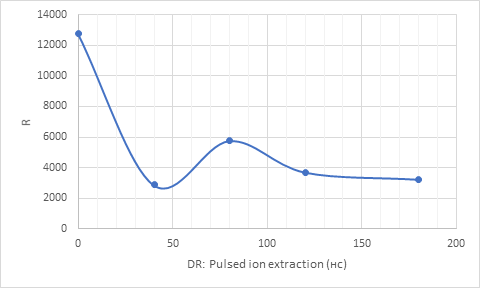
\includegraphics[width=1.2\linewidth]{6}
\caption{Зависимость разрешения пиков от времени включения ускоряющего потенциала с рефлектроном.}
\label{ris:experimcoded}
\end{minipage}
\end{center}
\end{figure}

\subsection{ Определение влияния подавления матрицы на масс-спектр}
Рассмотрели, как влияет параметр Deflection на масс-спектр. Сняли спектры при
различных значения этого параметра от 0 до 1200 Да с шагом 200 Да.
\begin{figure}[!h]
\begin{center}
\begin{minipage}[h]{0.4\linewidth}
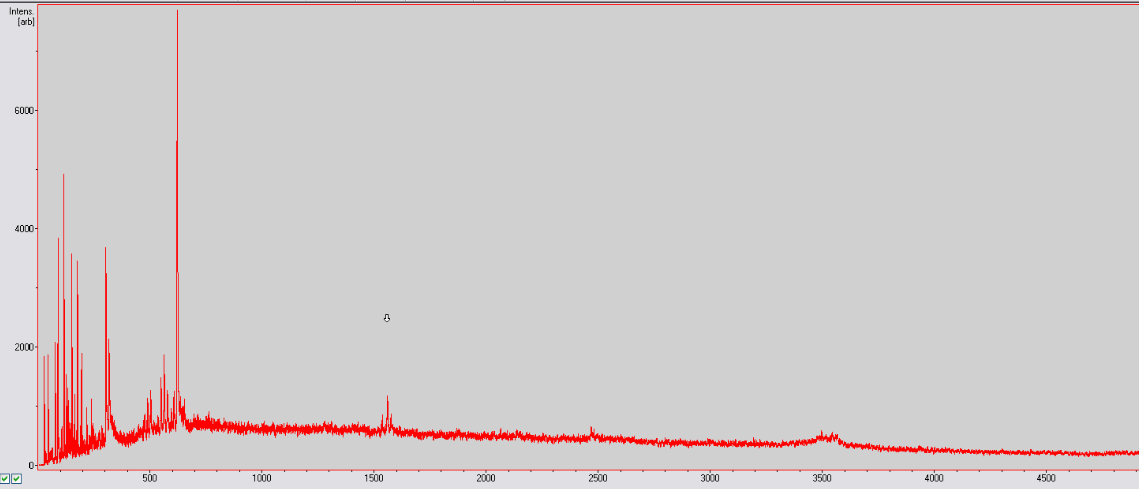
\includegraphics[width=1.2\linewidth]{26}
\caption{Спектр для 0 Да.} %% подпись к рисунку
\label{ris:experimoriginal} %% метка рисунка для ссылки на него
\end{minipage}
\hfill 
\begin{minipage}[h]{0.4\linewidth}
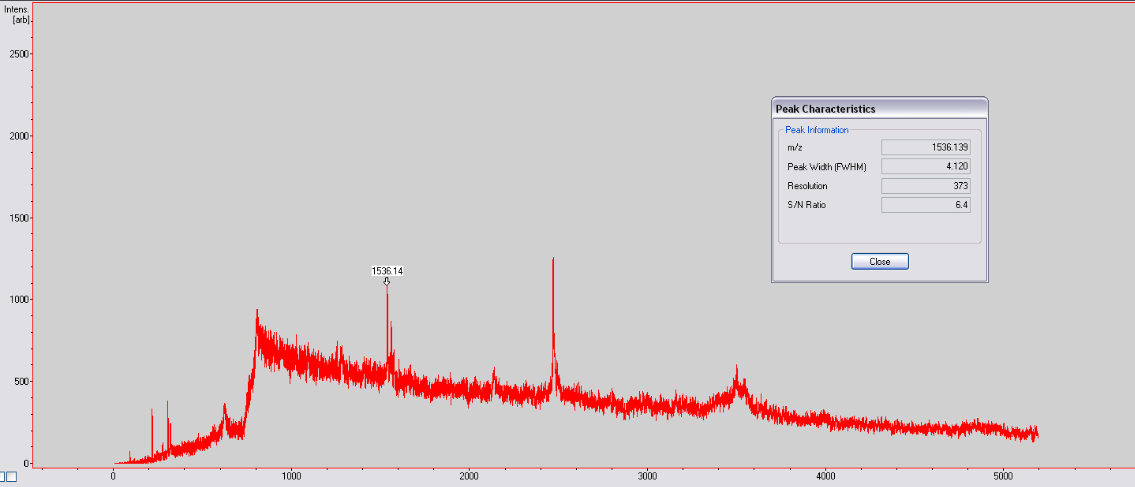
\includegraphics[width=1.2\linewidth]{27}
\caption{Спектр для 800 Да.}
\label{ris:experimcoded}
\end{minipage}
\end{center}
\end{figure}
\begin{figure}[!h]
\center{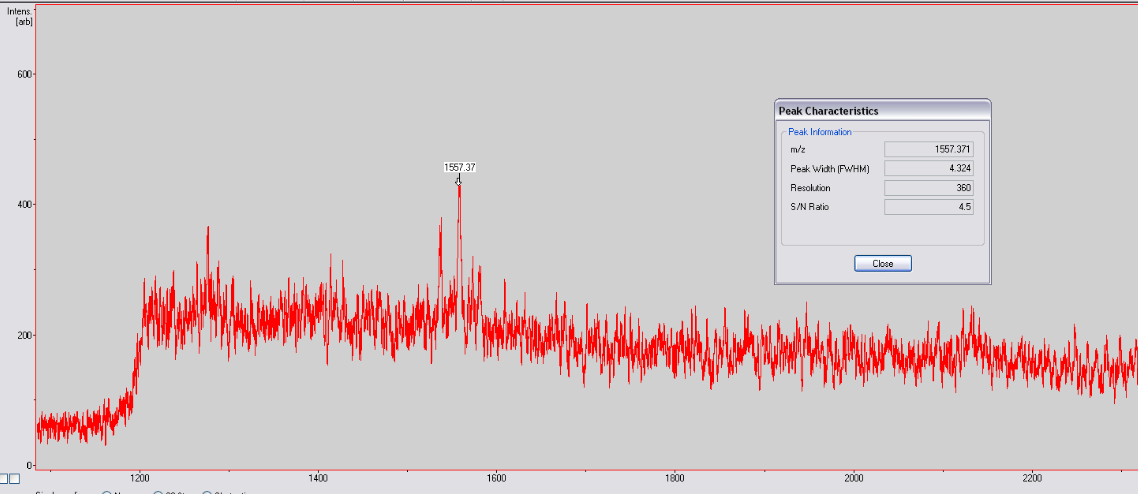
\includegraphics[width=14cm,height=6cm]{28}}
\caption{Спектр для 1200 Да.}
\label{ris:image}
\end{figure}

\begin{figure}[!h]
\begin{center}
\begin{minipage}[h]{0.4\linewidth}
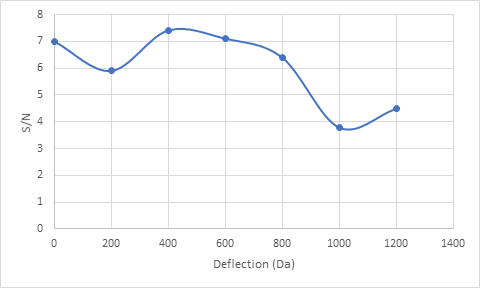
\includegraphics[width=1.2\linewidth]{29}
\caption{Зависимость значений S/N от параметра Deflection.} %% подпись к рисунку
\label{ris:experimoriginal} %% метка рисунка для ссылки на него
\end{minipage}
\hfill 
\begin{minipage}[h]{0.4\linewidth}
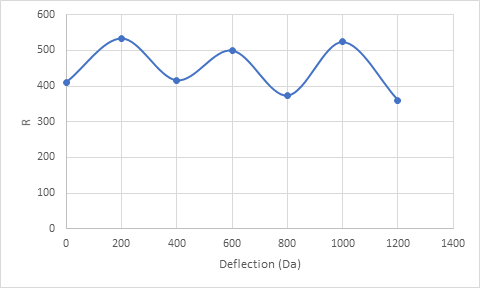
\includegraphics[width=1.2\linewidth]{30}
\caption{Зависимость разрешения пиков от от параметра Deflection.}
\label{ris:experimcoded}
\end{minipage}
\end{center}
\end{figure}

\section{Вывод}
Исходя из полученных данных, порог появления спектра соответствовал значению интенсивности излучения лазера 40 процентов в режиме измерений 
без рефлектрона. При использовании рефлектрона это значение повышается до 60 процентов, так как в таком режиме меньше ионов долетает до детектора.\\


Время задержки PIE не влияет на расплыв пика в некотором диапазоне. Однако при PIE больше 600 нс большая часть молекул откачивается форвакуумным насосом, что влияет на 
характеристики масс-спектра.\\
 
Полученных данных не достаточно для установления зависимости параметров масс-спектра от режима проведения измерений. Для установления зависимостей нужно произвести многократное повторение каждого измерения, чтобы говорить о статистической значимости выводов. 
Разброс значений, имеющихся на данный момент, можно объяснить как 
нелинейной зависимостью параметров спектра от режима эксперимента, 
так и неоднородностью распределения матрицы по поверхности пластины. 
Наличие фона на полученных масс-спектрах объясняется присутствием в смеси молекул матрицы, а также фрагментов аналита (даже при 
выключенном режиме фрагментации).
\section{Список литературы}
1. Основы MALDI TOF масс-спектрометрии: учеб.- метод. пособие
сост.: А.С. Воробьев, Е.С. Жванский, С.И. Пеков, К.В. Бочаров,
Д.А. Зубцов, И.А. Попов. - М.: МФТИ, 2018. - 38 с.


\end{flushleft}
\end{document}